\externaldocument{../3/chapter_modeling}
\externaldocument{../4/chapter_algorithm}
\startchapter{Dual\_trace Communication Analysis Prototype On Atlantis}
\label{chapter:newsol}
In this chapter, I present the design of the prototype of communication analysis from the dual\_trace. This prototype is implemented on Atlantis. It implemented some of the algorithms described in Chapter\ref{chapter:alo} as well as the user interfaces.

Atlantis as an assembly execution trace analysis environment, provides some functionalities that benefit the communication analysis of dual\_trace. Figure \ref{executable} shows the decoded information needed to identify a function call of interest from the trace. The functionality ``function inspect" of Atlantis provides this decoding functionality. In the function call event reconstruction algorithm, the parameters of a function call are retrieved from the memory state. The ``memory reconstruction" functionality of Atlantis which compute the memory state of the instruction line efficiently makes this retrieval easier. Moreover, the ``views synchronization" ability of Atlantis allows the user access various information at the same time when they are navigating and viewing the communication analysis result.

This prototype consists of four components: 1) declaring the function descriptors of the communication methods. 2) a view that can display both traces in the dual\_trace in parallel. 3)implementation of the communication analysis algorithms for stream extraction and communication identification. 4) a view for presenting the extracted streams and the identified communications from the dual\_trace.

The use cases presented in the following section depicts how to use these components to perform the communication analysis.

\section{Use Case}
To analyze a dual\_trace, the user need to perform the below operations in sequence:
\begin{itemize}
\item Open two traces in the parallel view(developed in this prototype)
\item Import the dynamic linked library files for each trace(existing functionality of Atlantis)
\item Perform the stream extraction or communication identification operations(developed in this prototype)
\item Inspect the operation results by navigating the analysis result from the communication view(developed in this prototype).
\end{itemize}

Two use cases of this prototype are designed. The use case shown in Table \ref{usecase1} is for stream exaction and the use case shown in Table \ref{usecase2} is for communication identification. 

\begin{table}[H]
  \centering
  \caption{Use Case 1: Extract Streams from the Dual\_trace}
  \label{usecase1}
  \begin{tabular}{|l|p{13cm}|}
      \hline
       \textbf{Name} & Analysis streams of a communication method from the Dual\_trace\\
       \hline
       \textbf{Description} & A user captured two assembly execution traces of two interacting programs and need to analysis them by extracting all communication streams of each of the traces and inspecting the extraction results \\
       \hline
              \textbf{Actor} & A Software Security Engineer \\
       \hline
       \textbf{Precondition} & The user has two assembly execution traces and the .dll files of the systems where the programs of the captured traces were running\\
       \hline
       \textbf{Main Course}& 1. The user declares the function descriptors for the communication methods of interest in the Json format setting file\\
        & 2. The user open one of the trace in Atlantis\\
       &  3. The user open the other trace as the dual\_trace of the first one\\
       & 4. The two opened traces are presented in the parallel view\\
       & 5. The user load the related .dll files for both opened trace\\
       & 6. The user select the operation ``Stream Extraction" in the ``Dual\_Trace Tool" menu.\\
       & 7. Atlantis prompt a dialog window giving the user all the communication methods in the function descriptor setting file as options\\
       & 8. The user select the communication methods which they want to analyze and click the ``OK" bottom\\
       & 9. Atlantis extract the streams for both traces and list the result in ``Communication view"\\
       & 10. The user expand the result in the ``Communication view"\\
       & 11. The user select one function call event in a stream and double click the entry\\
       & 12. Atlantis navigation to the corresponding instruction line in the trace and synchronize all other views\\
      \hline               
  \end{tabular}
\end{table}

\begin{table}[H]
  \centering
  \caption{Use Case 2: Identify Communications from the Dual\_trace}
  \label{usecase2}
  \begin{tabular}{|l|p{13cm}|}
      \hline
       \textbf{Name} & Identify communications of a communication method from the Dual\_trace\\
       \hline
       \textbf{Description} & A user captured two assembly execution traces of two interacting program and need to analysis them by identify all communications of the dual\_trace and inspecting the extraction results \\
       \hline
              \textbf{Actor} & A Software Security Engineer \\
       \hline
      \textbf{Precondition} & The user has two assembly execution traces and the .dll files of the systems where the programs of the captured traces were running\\
       \hline
       \textbf{Main Course}& 1. The user declares the function descriptors for the communication methods of interest in the Json format setting file\\
        & 2. The user open one of the trace in Atlantis\\
       &  3. The user open the other trace as the dual\_trace of the first one\\
       & 4. The two opened traces are presented in the parallel view\\
       & 5. The user load the related .dll files for both opened trace\\
       & 6. The user select the operation ``Communication Identification" in the ``Dual\_Trace Tool" menu\\
      & 7. Atlantis prompt a dialog window giving the user all the communication methods in the function descriptor setting file as options\\
       & 8. The user select the communication methods which they want to analyze and click the ``OK" bottom\\
       & 9. Atlantis identify the communications of the dual\_trace and list the result in ``Communication view"\\
       & 10. The user expand the result in the ``Communication view"\\
       & 11. The user select one function call event in a stream and double click the entry\\
       & 12. Atlantis navigation to the corresponding instruction line in the trace and synchronize all other views\\
      \hline               
  \end{tabular}
\end{table}

\section{Declaring of the Function Descriptors}\label{functionset}
In Section \ref{cdesc}, I defined a function descriptor as a set of function descriptions for a communication method. Each function description consist with four elements: $fdesc = \lbrace name, type, inparamdesc, outparamdesc \rbrace$. $name$ is the function name, $type$ can be $open$, $close$, $send$ and $receive$, $inparamdesc$ and $outparamdesc$ are the descriptions for the input and output parameters of interest(you might not care for all parameters). The communication analysis approach depicted in Chapter \ref{chapter:alo} can identify the communications described by the function descriptor from the dual\_trace.

However, the function descriptor for a communication method can be different depending on the implementation of the communication method in a program. Rather than hard coding the function descriptors for the communication methods, the prototype loads the function descriptors from a configuration file. A default template is given for reference. This template is generated by Atlantis when it was launched and stored in the .tmp folder of the trace analysis project. The users can modify this template as to the communication methods of interest. The default template example can be find in Appendix \ref{funcset}.

The function descriptors in this setting file will be the input for the stream extraction and communication identification features. When the user use these two features, the list of the communication methods provided in the function descriptor configuration file will be presented to them. They can select one or more communication methods to be analyzed. 

In the following subsections, function descriptor examples are presented for reference. Other function descriptors can be obtained by following the same process as developing the function descriptor examples.

\subsection{Communication Methods' Implementation in Windows}\label{windows}
Learning the implementation of a communication is necessary to obtain the function descriptor of the communication method. In this section, I present the result of investigation about the implementation of these four communication methods: Named Pipe, Message Queue, TCP and UDP in Windows. In the investigation, I reviewed the Windows APIs of the communication methods and their example code. By doing so, I obtained the function descriptors of these methods. 

Windows API set is very sophisticated. Moreover, multiple solutions are provided to fulfil a communication method. It is unfeasible to enumerate all solutions for each communication method. I only investigated the most basic usage provided in Windows documentation. For each communication method, a function descriptor with a list of system function descriptions is provided for reference. The functions in the descriptors are supported in most Windows operating systems, such as Windows 8, Window 7. The provided function descriptor of a communication method should only be considered as an example for that communication method. With the understanding of this, it should be fairly easy to obtain the function descriptors for other solutions of that communication method or other communication methods. 

Note that, the instances of the descriptors only demonstrate Windows C++ APIs. But the idea of the function descriptor is generalizable to other operating systems with the effort of understanding the APIs of those operating systems.

\subsubsection{Windows Calling Convention}
It is important to know the Windows calling convention for this research. The communication analysis from a dual\_trace in assembly level relies not only on the system function names but also the key parameter values and the return values. In the assembly level execution traces, the parameter and return values are captured in the memory changes and register changes of the instructions but without any explicit information indicating which registers or memory addresses are holding this parameters. The calling convention tells us where the parameters are stored. So that we can find them in the memory state while emulating the execution of the trace. Each operating system has their own calling convention for different programming languages. I used dual\_trace of Microsoft* x64 programs for case study in this research. The Microsoft* x64 calling convention is listed in Appendix \ref{convention} as example.

\subsubsection{Named Pipes}
In Windows, a named pipe is a communication method between one server and one or more clients. The pipe has a name and can be one-way or duplex. Both the server and clients can read or write into the pipe.\cite{WinNamedpipe} In this work, I only consider one server versus one client communication.(One server to multiple clients scenario can always be divided into multiple ``one server and one client" communications thanks to the characteristic that each client and server communication has a separate conduit.) The server and client are endpoints in the communication. We call the server ``server endpoint" while the client ``client endpoint".  The server endpoint and client endpoint of a named pipe share the same pipe name, but each endpoint has its own buffers and handles. 

There are two modes for data transfer in the named pipe communication method, synchronous and asynchronous. Modes affect the functions used to complete the send and receive operations. The function descriptors for both synchronous mode and asynchronous mode are provided. The create channel functions for both modes are the same while the mode is indicated by an input parameter. The functions for send and receive message are also the same for both cases. However, the operations of the send and receive functions are different for different modes. In addition, an extra function \textit{GetOverlappedResult} is being called to check if the sending or receiving operation finish, the output message will be stored in the overlap structure whose memory address saved in the function's output parameter OverlapStruct. Table \ref{namesyn} is the function descriptor for synchronous mode while Table \ref{nameasyn} is the function descriptor asynchronous mode of Named pipe.

\begin{table}[H]
  \centering
  \caption{Function Descriptor for Synchronous Named Pipe}
  \label{namesyn}
  \begin{tabular}{|l|l|l|l|l|l|l|l|}
\hline
             \multirow{2}{*}{{\textbf{Name}}} & \multirow{2}{*}{{\textbf{Type}}} & \multicolumn{3}{c|}{\textbf{Input Parameters Description}} & \multicolumn{3}{c|}{\textbf{Output Parameters Description}} \\
              \cline{3-8} 
             & & \textbf{Name}& \textbf{Register} & \textbf{Addr/Val} & \textbf{Name}& \textbf{Register} &  \textbf{Addr/Val}  \\
             \hline
      CreateNamedPipe
       &open & FileName & RCX  & Addr &  Handle & RAX & Val\\
      \hline         
      CreateFile
       &open & FileName & RCX & Addr&  Handle & RAX & Val\\ 
      \hline              
      \multirow{2}{*}{WriteFile}
       &\multirow{2}{*}{send} &  Handle & RCX & Val & Length & R9 &Val\\
        \cline{3-8} 
       & & SendBuf & RDX & Addr & RetVal& RAX & Val\\
      \hline            
      \multirow{2}{*}{ReadFile}
       &\multirow{2}{*}{receive} &  Handle & RCX & Val& Length &R9 & Val\\
        \cline{3-8} 
       & & RecvBuf & RDX  & Addr & RetVal& RAX & Val\\
      \hline            
      CloseHandle &
       close &  Handle & RCX & Val & RetVal& RAX & Val\\
      \hline            
      DisconnectNamedPipe &
      close &  Handle & RCX & Val & RetVal& RAX & Val\\
      \hline               
  \end{tabular}
\end{table}

\begin{table}[H]
  \centering
  \caption{Function Descriptor for Asynchronous Named Pipe}
  \label{nameasyn}
\begin{tabular}{|l|l|l|l|l|l|l|l|}
\hline
             \multirow{2}{*}{{\textbf{Name}}} & \multirow{2}{*}{{\textbf{Type}}} & \multicolumn{3}{c|}{\textbf{Input Parameters Description}} & \multicolumn{3}{c|}{\textbf{Output Parameters Description}} \\
              \cline{3-8} 
             & & \textbf{Name}& \textbf{Register} & \textbf{Addr/Val} & \textbf{Name}& \textbf{Register} &  \textbf{Addr/Val}  \\
             \hline
      CreateNamedPipe
       &open & FileName & RCX  & Addr &  Handle & RAX & Val\\
      \hline         
      CreateFile
       &open & FileName & RCX & Addr&  Handle & RAX & Val\\ 
      \hline              
      \multirow{2}{*}{WriteFile}
       &\multirow{2}{*}{send} &  Handle & RCX & Val & Length & R9 & Val\\
        \cline{3-8} 
       & & SendBuf & RDX & Addr & RetVal& RAX & Val\\
      \hline            
      \multirow{2}{*}{ReadFile}
       &\multirow{2}{*}{receive} &  Handle & RCX & Val& Length & R9 & Val\\
        \cline{3-8} 
       & & RecvBuf & RDX  & Addr & RetVal& RAX & Val\\
      \hline    
           \multirow{2}{*}{GetOverlappedResult} &
       \multirow{2}{*}{receive} &  \multirow{2}{*}{Handle} & \multirow{2}{*}{RCX} & \multirow{2}{*}{Val} &OverlapStruct &RDX & Addr\\
               \cline{6-8} 
       & &  &   &  & RetVal& RAX & Val\\
      \hline     
      CloseHandle &
       close &  Handle & RCX & Val & RetVal& RAX & Val\\
      \hline            
      DisconnectNamedPipe &
      close &  Handle & RCX & Val & RetVal& RAX & Val\\
      \hline               
  \end{tabular}  
\end{table}

\subsubsection{Message Queue}
Similar to Named Pipe, Message Queue's implementation in Windows also has two modes, synchronous and asynchronous. The asynchronous mode is also further divided into two operations: one with callback function while the other without. With the callback function, the callback function would be called when the send or receive operations finish. Without a callback function, the general function \textit{MQGetOverlappedResult} should be called by the endpoints to check if the message sending or receiving operation finish, the parameter in RCX of this function call is a structure consist of the handle as an input parameter and the overlap structure as an output parameter. Table \ref{msmqsynfunctions} is the function descriptor for synchronous mode while Table \ref{msmqasynfunctions} is the function descriptor for the asynchronous mode without callback. I did not exemplify the with callback function, since the specific callback function and its parameters need to be known for developing this the function descriptor.

\begin{table}[H]
  \centering
  \caption{Function Descriptor for Synchronous Message Queue}
  \label{msmqsynfunctions}
\begin{tabular}{|l|l|l|l|l|l|l|l|}
\hline
             \multirow{2}{*}{{\textbf{Name}}} & \multirow{2}{*}{{\textbf{Type}}} & \multicolumn{3}{c|}{\textbf{Input Parameter Description}} & \multicolumn{3}{c|}{\textbf{Output Parameter Description}} \\
              \cline{3-8} 
             & & \textbf{Name}& \textbf{Register} & \textbf{Addr/Val} & \textbf{Name}& \textbf{Register} &  \textbf{Addr/Val}  \\
             \hline
      MQOpenQueue
       &open & QueueName & RCX  & Addr &  Handle & RAX & Val\\
      \hline                     
      \multirow{2}{*}{MQSendMessage}
       &\multirow{2}{*}{send} &  Handle & RCX & Val & \multirow{2}{*}{RetVal} & \multirow{2}{*}{RAX}  & \multirow{2}{*}{Val} \\
       \cline{3-5}
      & & MessStruct& RDX&Addr &   &  &  \\
      \hline            
      \multirow{2}{*}{MQReceiveMessage}
       &\multirow{2}{*}{receive}&  \multirow{2}{*}{Handle} & \multirow{2}{*}{RCX} & \multirow{2}{*}{Val}& MessStruct& RDX&Addr\\
              \cline{6-8}
      & & & & & RetVal & RAX & Val\\
      \hline       
      MQCloseQueue &
       close &  Handle & RCX & Val & RetVal & RAX & Val\\
      \hline                          
  \end{tabular}   
\end{table}

\begin{table}[H]
  \centering
  \caption{Function Descriptor for Asynchronous Message Queue}
  \label{msmqasynfunctions}
\begin{tabular}{|l|l|l|l|l|l|l|l|}
\hline
             \multirow{2}{*}{{\textbf{Name}}} & \multirow{2}{*}{{\textbf{Type}}} & \multicolumn{3}{c|}{\textbf{Input Parameter Description}} & \multicolumn{3}{c|}{\textbf{Output Parameter Description}} \\
              \cline{3-8} 
             & & \textbf{Name}& \textbf{Register} & \textbf{Addr/Val} & \textbf{Name}& \textbf{Register} &  \textbf{Addr/Val}  \\
             \hline
      MQOpenQueue
       &open & QueueName & RCX  & Addr &  Handle & RAX & Val\\
      \hline                     
      \multirow{2}{*}{MQSendMessage}
       &\multirow{2}{*}{send} &  Handle & RCX & Val & \multirow{2}{*}{RetVal} & \multirow{2}{*}{RAX}  & \multirow{2}{*}{Val} \\
       \cline{3-5}
      & & MessStruct& RDX&Addr &   &  &  \\
      \hline            
           \multirow{2}{*}{MQReceiveMessage}
       &\multirow{2}{*}{receive}&  \multirow{2}{*}{Handle} & \multirow{2}{*}{RCX} & \multirow{2}{*}{Val}& MessStruct& RDX&Addr\\
              \cline{6-8}
      & & & & & RetVal & RAX & Val\\
      \hline    
      \multirow{2}{*}{MQGetOverlapResult} &
       \multirow{2}{*}{receive} &  \multirow{2}{*}{Handle} & \multirow{2}{*}{RCX} & \multirow{2}{*}{Addr} & Overlapstr& RCX&Addr\\
                     \cline{6-8}
      & & & & & RetVal & RAX & Val\\
      \hline      
      MQCloseQueue &
       close &  Handle & RCX & Val & RetVal & RAX & Val\\
      \hline                          
  \end{tabular}   
\end{table}


    
\subsubsection{TCP and UDP}
In Windows programming, these two methods share the same set of APIs regardless the input parameter values and operation behavior are different. In the Windows socket solution, one of the two endpoints is the server while the other one is the client. Table \ref{tcpupdfunctions} is the function descriptor for UDP or TCP communication. 

\begin{table}[H]
  \centering
  \caption{Function Descriptor for for TCP and UDP}
  \label{tcpupdfunctions}
\begin{tabular}{|l|l|l|l|l|l|l|l|}
\hline
             \multirow{2}{*}{{\textbf{Name}}} & \multirow{2}{*}{{\textbf{Type}}} & \multicolumn{3}{c|}{\textbf{Input Parameters Description}} & \multicolumn{3}{c|}{\textbf{Output Parameters Description}} \\
              \cline{3-8} 
             & & \textbf{Name}& \textbf{Register} & \textbf{Addr/Val} & \textbf{Name}& \textbf{Register} &  \textbf{Addr/Val}  \\
             \hline
      socket
       &open &  &   &  &  Socket & RAX & Val\\ 
      \hline
      bind
       &open & Socket &  RCX & Val &  ServerAddrAndPort & RDX & Addr\\
      \hline   
            connect
       &open & Socket &  RCX & Val &  ServerAddrAndPort & RDX & Addr\\
      \hline   
     accept
       &open &  ListenSocket & RCX & Val & ConnectSocket & RAX & Val\\
      \hline                    
      \multirow{2}{*}{send}
       &\multirow{2}{*}{send} &  Handle & RCX & Val & \multirow{2}{*}{RetVal}& \multirow{2}{*}{RAX} & \multirow{2}{*}{Val} \\
       \cline{3-5}
      & & SendBuf& RDX&Addr &  &  & \\
      \hline            
      \multirow{2}{*}{recv}
       &\multirow{2}{*}{receive}&  \multirow{2}{*}{Handle} & \multirow{2}{*}{RCX} & \multirow{2}{*}{Val}& RecvBuf& RDX&Addr\\
       \cline{6-8}
      & &  &   &  &  RetVal & RAX & Val\\ 
      \hline      
      closesocket &
       close &  Handle & RCX & Val & RetVal & RAX & Val\\
      \hline                          
  \end{tabular}    
\end{table}

\section{Parallel Trace View For Dual\_Trace}
The dual\_trace consists of two execution traces which are interacting with each other. Presenting them in the parallel trace view makes the analysis for the user much easier. A parallel trace view implemented in Atlantis can display two execution traces side by side. To open the parallel trace view, the user need to open one trace as the normal one and the other as the dual\_trace of the active(opened) one. A new menu option in the project navigation view of Atlantis was added to open the second trace as the dual\_trace of the active one. The implementation of the parallel view takes advantage of the existing SWT of Eclipse plug-in development. The detail of the implementation can be found in Appendix \ref{parallelview}. Figure \ref{opendualtracemenu} shows the ``Open as Dual\_Trace" menu option and Figure \ref{parallelview} shows the parallel trace view with two traces displaying side by side.

\begin{figure}[H]
\centerline{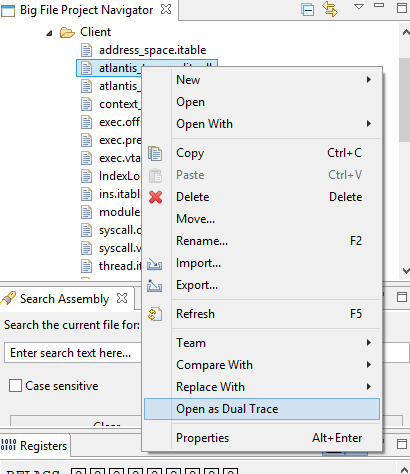
\includegraphics[scale=0.4]{Figures/opendualtracemenu}}
 \caption{Menu Item for opening Dual\_trace}
\label{opendualtracemenu}
\end{figure}

\begin{figure}[H]
\centerline{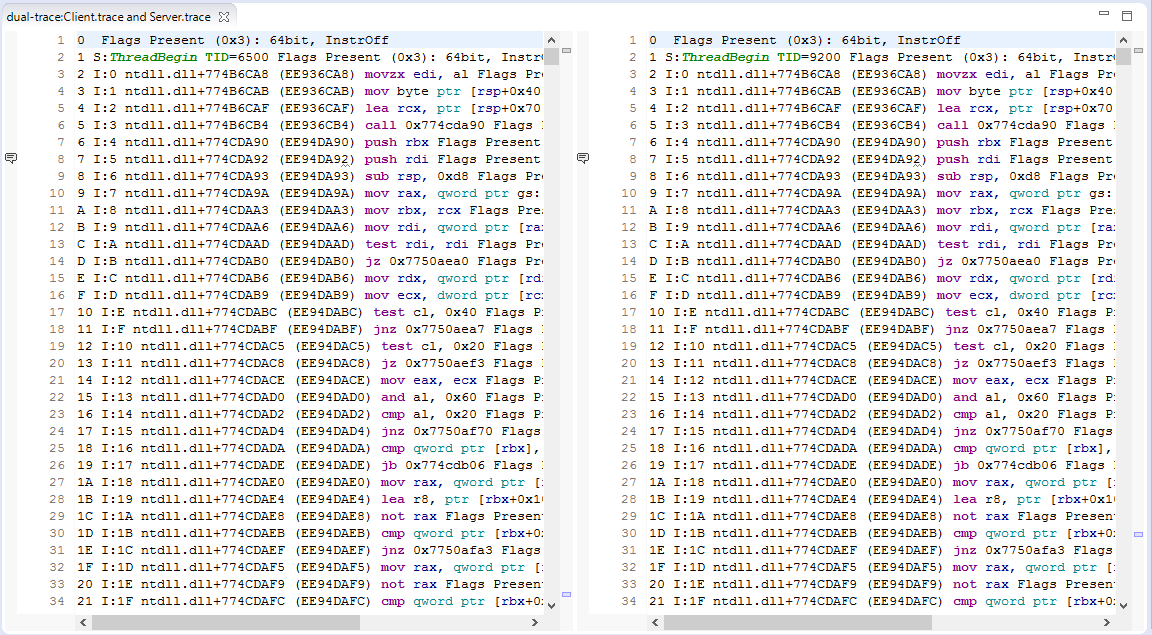
\includegraphics[scale=0.6]{Figures/paralleleditor}}
 \caption{Parallel Trace View}
\label{parallelview}
\end{figure}

\section{Implementation of the Communication Analysis Algorithms}
The implementation is divided into two parts. The first part is stream extraction. It implements the first section of the overall process of the communication analysis as shown in Figure \ref{overviewintwo} and present the extracted streams of both traces in the dual\_trace to the user. The second part is stream extraction. It implements the whole process of the communication analysis as shown in Figure \ref{overviewintwo} and present the identified communications of the dual\_trace to the user.

\begin{figure}[H]
\centerline{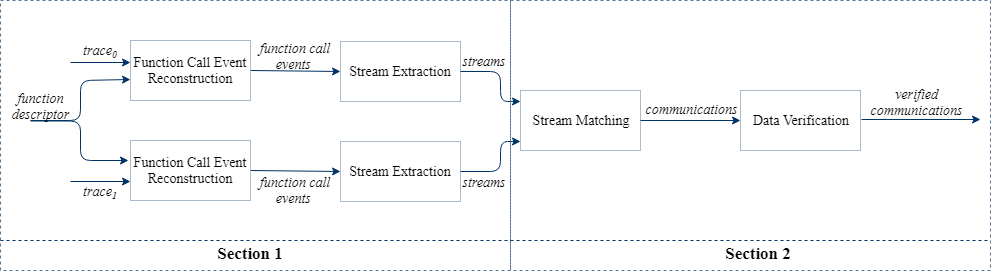
\includegraphics[scale=0.55]{Figures/overviewintwo}}
\caption{Process of the Communication Analysis from a Dual\_trace Separated in Two Sections}
\label{overviewintwo}
\end{figure}

The implementation relies on the existing ``function inspect" feature of Atlantis. The called functions' name can be inspected  by  search of the symbolic name in the executable binary or any DLLs which used by the program at the time when it is traced. By importing the DLLs and executable binary, Atlantis can recognize the function call from the execution trace by the function names. Therefore the corresponding Dlls or executable binaries for both traces in the dual\_trace have to be loaded into Atlantis before conducting the identification.

A new menu ``Dual\_trace Tool" with three menu options is designed for these two operations. In this menu, ``Stream Extraction" is for the operation of stream extraction and ``Communication Identification" is for the operation of communication identification. For both of these two operation ``Load Library Exports" has to be run before for both traces. Currently, the ``Load library export"  operation can only load libraries for the trace in the active trace view. So ``Load library export"  in the menu has to be run twice separately for each trace of the dual\_trace.  Figure\ref{dualtracetoolmenu} shows this new menu in Atlantis. When the user perform ``Stream Extraction" or ``Communication Identification", there will be a prompt dialog window as shown in Figure \ref{methods} which asks the user what communication methods they want to analyze from the dual\_trace. This list is provided by the configuration file I mention in Section \ref{functionset}. The user can select one or multiple methods. Atlantis will perform the operations after the user select and confirm the communication methods.

\begin{figure}[H]
\centerline{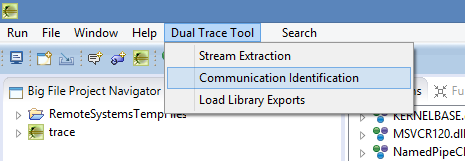
\includegraphics{Figures/dualtracetoolmenu}}
 \caption{Dual\_trace Tool Menu}
\label{dualtracetoolmenu}
\end{figure}

\begin{figure}[H]
\centerline{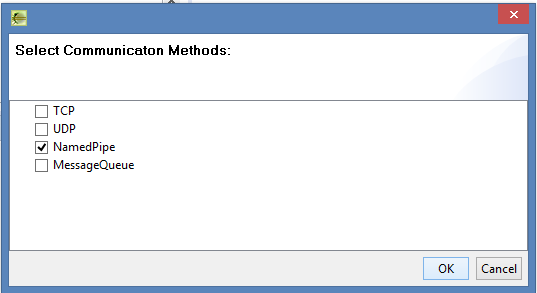
\includegraphics[scale=0.8]{Figures/methods}}
 \caption{Prompt Dialog for Communication Selection}
\label{methods}
\end{figure}

\section{View of Extracted Streams and Identified Communications}
A new view named ``Communication View" is designed for presenting the result of the extracted streams and the identified communications. Since the user can have multiple selection for communication methods of interest, the output result contains all the streams or communications of all selected communication methods and the results are clustered by methods. There are two sub tables in this view, the left one is for presenting the extracted streams while the left one is for presenting identified communications. The reason for putting this two result in the same view is for easy access to and comparison of the data for the users. Figure \ref{idenview} shows this view with both extracted streams result and identified communication result in it. Each time when the user rerun the operations the result in the corresponding table will be refreshed to show only the latest result of that operation. But the other table will not be affected. For example, if the user run the ``Stream Extraction" operation first, the extracted streams will show on the left table of the view. And then the user perform the ``communication Identification" operation, the identified communications result will be shown on the right table while the left one still holding the last stream extraction result.

\begin{figure}[H]
\centerline{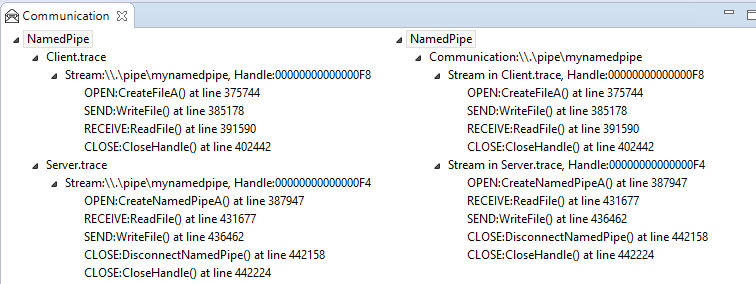
\includegraphics[scale=0.7]{Figures/idenview}}
 \caption{Communication View for Result}
\label{idenview}
\end{figure}

Atlantis is a analysis environment that has various views to allow user access to different information from the trace, such as the memory and register state of the current instruction line. Moreover, these views synchronize automatically with the trace view. These functionality and information also benefit the communication analysis of the dual\_trace. Providing the user a way to navigate from the result of the extracted streams and the identified communications to the trace views allows them to take advantage of the current existing functionality of Atlantis and make their analysis of the dual\_trace more efficient.

The results presented in the tables of the Communication view contains contains all the function call events, each event entry is a function call in the corresponding trace. The functions were called at function call line and all the inputs of the function calls can be recovered from the memory state of this instruction line. The functions returned at the return instruction lines, all the outputs of the function calls can be recovered in the memory state of the the return instruction line. From the event entries, this implementation provide two different ways for the user to navigate back to where the function begins and ends. When the user ``double click" on an entry, it will bring the user to the start line of the function in the corresponding trace view. When the user right click on the event entry, a prompted menu with the option ``Go To Line of Function End" will show up as in Figure \ref{gotoend}. Clicking on this option will bring the user to the return line of this function in the trace view. All other opened views of Atlantis update immediately with this navigation. 

\begin{figure}[H]
\centerline{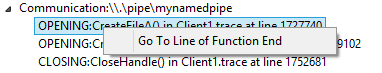
\includegraphics{Figures/gotoend}}
 \caption{Right Click Menu on Event Entry}
\label{gotoend}
\end{figure}

Moreover, the ``remove" option as shown in Figure \ref{remove} in the right click menu on the ``stream“ or ``communication" entries is provided for the user to remove the selected ``stream" or ``communication" entry. This provides the user the flexibility to get rid of the data that they don't care.

\begin{figure}[H]
\centerline{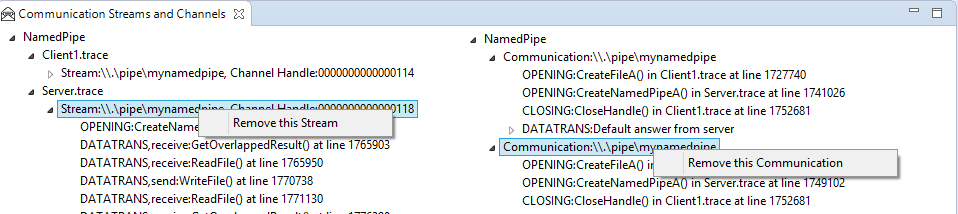
\includegraphics[scale=0.7]{Figures/remove}}
 \caption{Right Click Menu on Event Entry}
\label{remove}
\end{figure}

